%\documentclass[compress,t,11pt]{beamer}
\documentclass[handout,compress,t,11pt]{beamer}
\usetheme[]{metropolis}           % Use metropolis theme
\usefonttheme{serif}
\definecolor[named]{Gray}{RGB}{111,112,114}
\definecolor[named]{DarkGray}{RGB}{48,48,48}
\definecolor[named]{Cardinal}{RGB}{179,22,34}
\usepackage[T1]{fontenc}
\usepackage[altbullet]{lucidabr}
\usepackage{textcomp}
\usepackage{upquote} % needed to make straight quotes work in listings
\usepackage{listgolang}
\usepackage{mathtools}
\usepackage{comment}
\usepackage{tikz}
\usepackage{tikzsymbols}
 \usetikzlibrary{trees,shapes,plotmarks,arrows,er,automata,petri,topaths,positioning}
\usepackage{pifont}
\usepackage{clrscode}
\usepackage{setspace}
\usepackage{soul}
\usepackage{hyperref}
\usepackage{calc}  
\usepackage{enumitem}  
\setlist[itemize]{label={\color{Gray}\textbullet}}

\setbeamercolor{palette primary}{fg=white,bg=Cardinal}
\setbeamercolor{palette secondary}{fg=white,bg=Gray}
\setbeamercolor{palette tertiary}{fg=white,bg=Cardinal}
\setbeamercolor{palette quaternary}{fg=white,bg=Gray}
\setbeamercolor{palette sidebar primary}{fg=white,bg=Cardinal}
\setbeamercolor{palette sidebar secondary}{fg=white,bg=Gray}
\setbeamercolor*{titlelike}{fg=Cardinal}
\setbeamercolor{structure}{fg=Gray}
\setbeamercolor{title separator}{fg=Cardinal}
\setbeamercolor{alerted text}{fg=Cardinal}
\setbeamercolor{reversed}{fg=Cardinal,bg=black}

\newcommand{\card}[1]{\ensuremath{\left|#1\right|}}
\newcommand{\norm}[1]{\ensuremath{\|#1\|}}

\title[Programming in Go]{\bf Programming in Go\\ Lesson 0: The Very Basics}
\author{Matt Holiday} 
\institute[CP]{Cardinal Peak}
\date{24 February 2019} 
%\titlegraphic{\hfill
\includegraphics[width=.25\textwidth,height=.25\textheight]{cp-logo-2x.png}}
\titlegraphic{
\begin{tikzpicture}[overlay, remember picture,scale=0.4]
\node[at=(current page.north east), anchor=north east] (a) {};
\node[below left = 0.1cm and 0.1cm of a] (b)
{
\includegraphics[width=.25\textwidth,height=.25\textheight]{cp-logo-2x.png}};
\node[below left=2.56cm and 2.9cm of b]
{
\includegraphics[width=.1\textwidth]{go-logo.png}};
\end{tikzpicture}}

\setbeamerfont{footline}{series=\bfseries\selectfont}
\setbeamersize{text margin left=12pt,text margin right=12pt}
\linespread{1.0}
\metroset{block=fill}

\hypersetup{
    colorlinks=true,
    linkcolor=Cardinal,
    filecolor=magenta,      
    urlcolor=blue,
}

\begin{document}
\frame{\titlepage} 

%\section{Introduction}
\begin{frame}[fragile]
    \frametitle{The Book}
    Hereinafter referred to as {\em GOPL} \par
    \vspace{0.4\baselineskip}
    \begin{minipage}[c]{0.55\textwidth}
        I will be taking exercise material 
        from this book \par
        \vspace{\baselineskip}
        
    Amazon paper: \$28 \par
    \vspace{\baselineskip}
    \verb|informit.com| PDF: \$19 \\
    (with coupon \verb|IUGD45|)
    \end{minipage}%
    \begin{minipage}[c]{0.35\textwidth}
        \vspace{0.5\baselineskip}
        \hfill 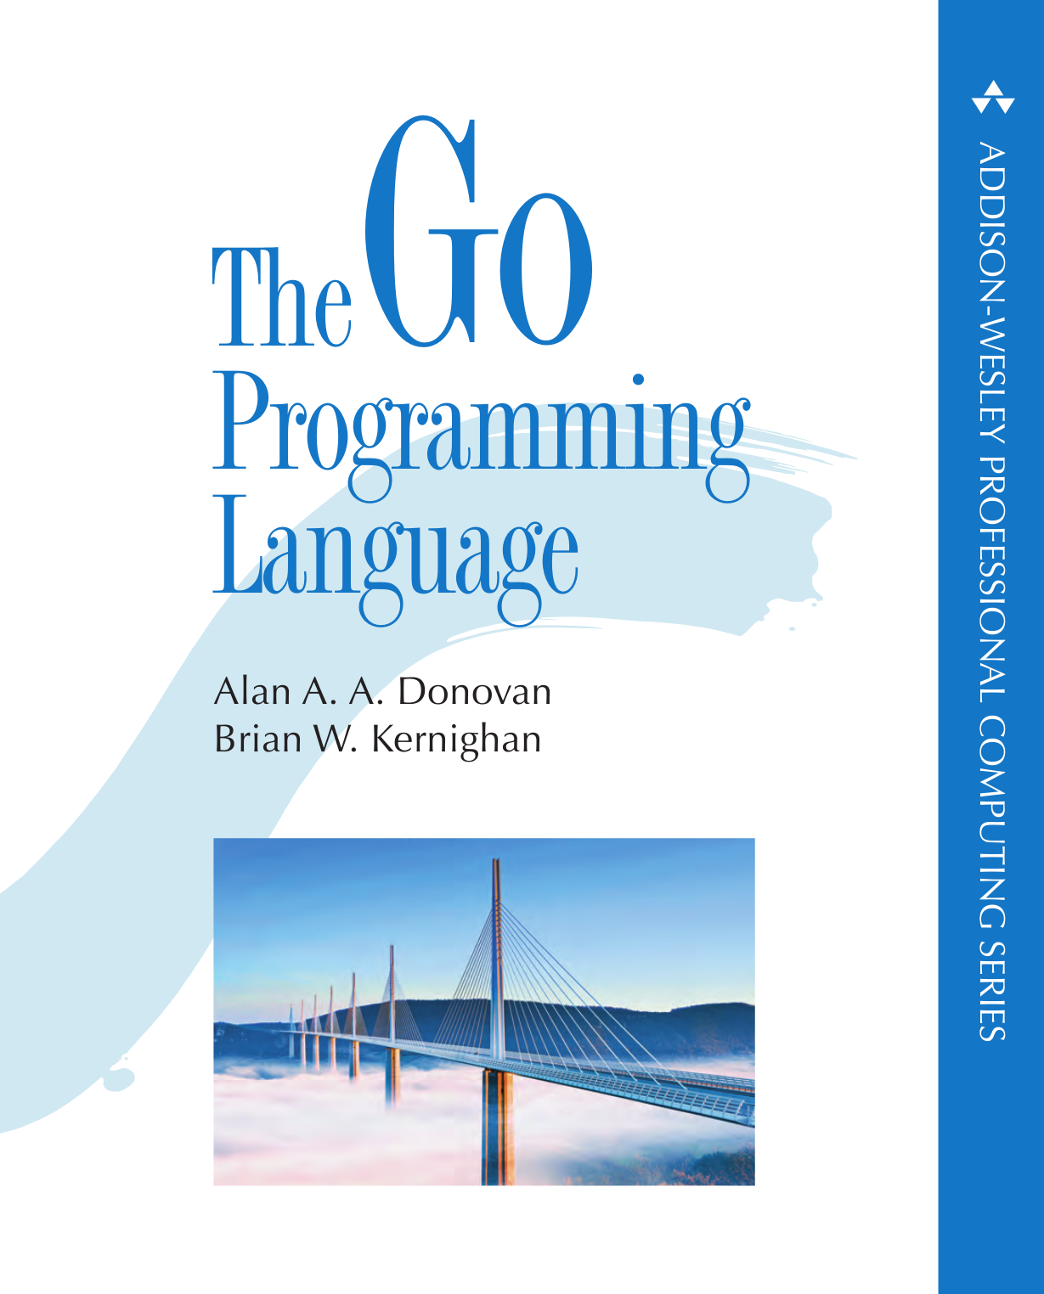
\includegraphics[width=0.85\textwidth,height=.5\textheight]{cover}
    \end{minipage} \par
    \vspace{2\baselineskip}
    ``Anything with Brian Kernighan's name on it is worth reading.'' \\--- Matt Holiday
\end{frame}

\begin{frame}[fragile]
\frametitle{Hello, world!}
What the simplest program looks like:
\begin{golang}
package main

import "fmt"

func main() {
    fmt.Println("Hello, world!")
}
\end{golang}
\end{frame}

\begin{frame}[fragile]
\frametitle{Hello, world!}
What the simplest program looks like:
\begin{golang}
package main

import "fmt"

func main() {
    fmt.Println("Hello, world!")
}
\end{golang}
    \vspace{0.5\baselineskip}
The program must have a \verb|main| function to get started \par
    \vspace{0.5\baselineskip}
The main function must live in package \verb|main| because everything
must be in some package \par
    \vspace{0.5\baselineskip}
Anything we use from another package must be {\em imported}
\end{frame}

\begin{frame}[fragile]
\frametitle{Hello, world!}
What the simplest program looks like:
\begin{golang}
package main

import "fmt"

func main() {
    fmt.Println("Hello, world!")
}
\end{golang}
    \vspace{0.5\baselineskip}
The body of \verb|main| is in curly braces \verb|{}| with just a
{\em function call} to print output to the console \par
    \vspace{0.5\baselineskip}
Package \verb|fmt| is where we find utilities for formatted output \par
    \vspace{0.5\baselineskip}
\verb|Println| prints its {\em arguments} and terminates the line
\end{frame}

\begin{frame}[fragile]
\frametitle{Hello, playground!}
Simple programs run at the \href{https://play.golang.org}{Go playground}
    \vspace{-0.4\baselineskip}
\begin{center}
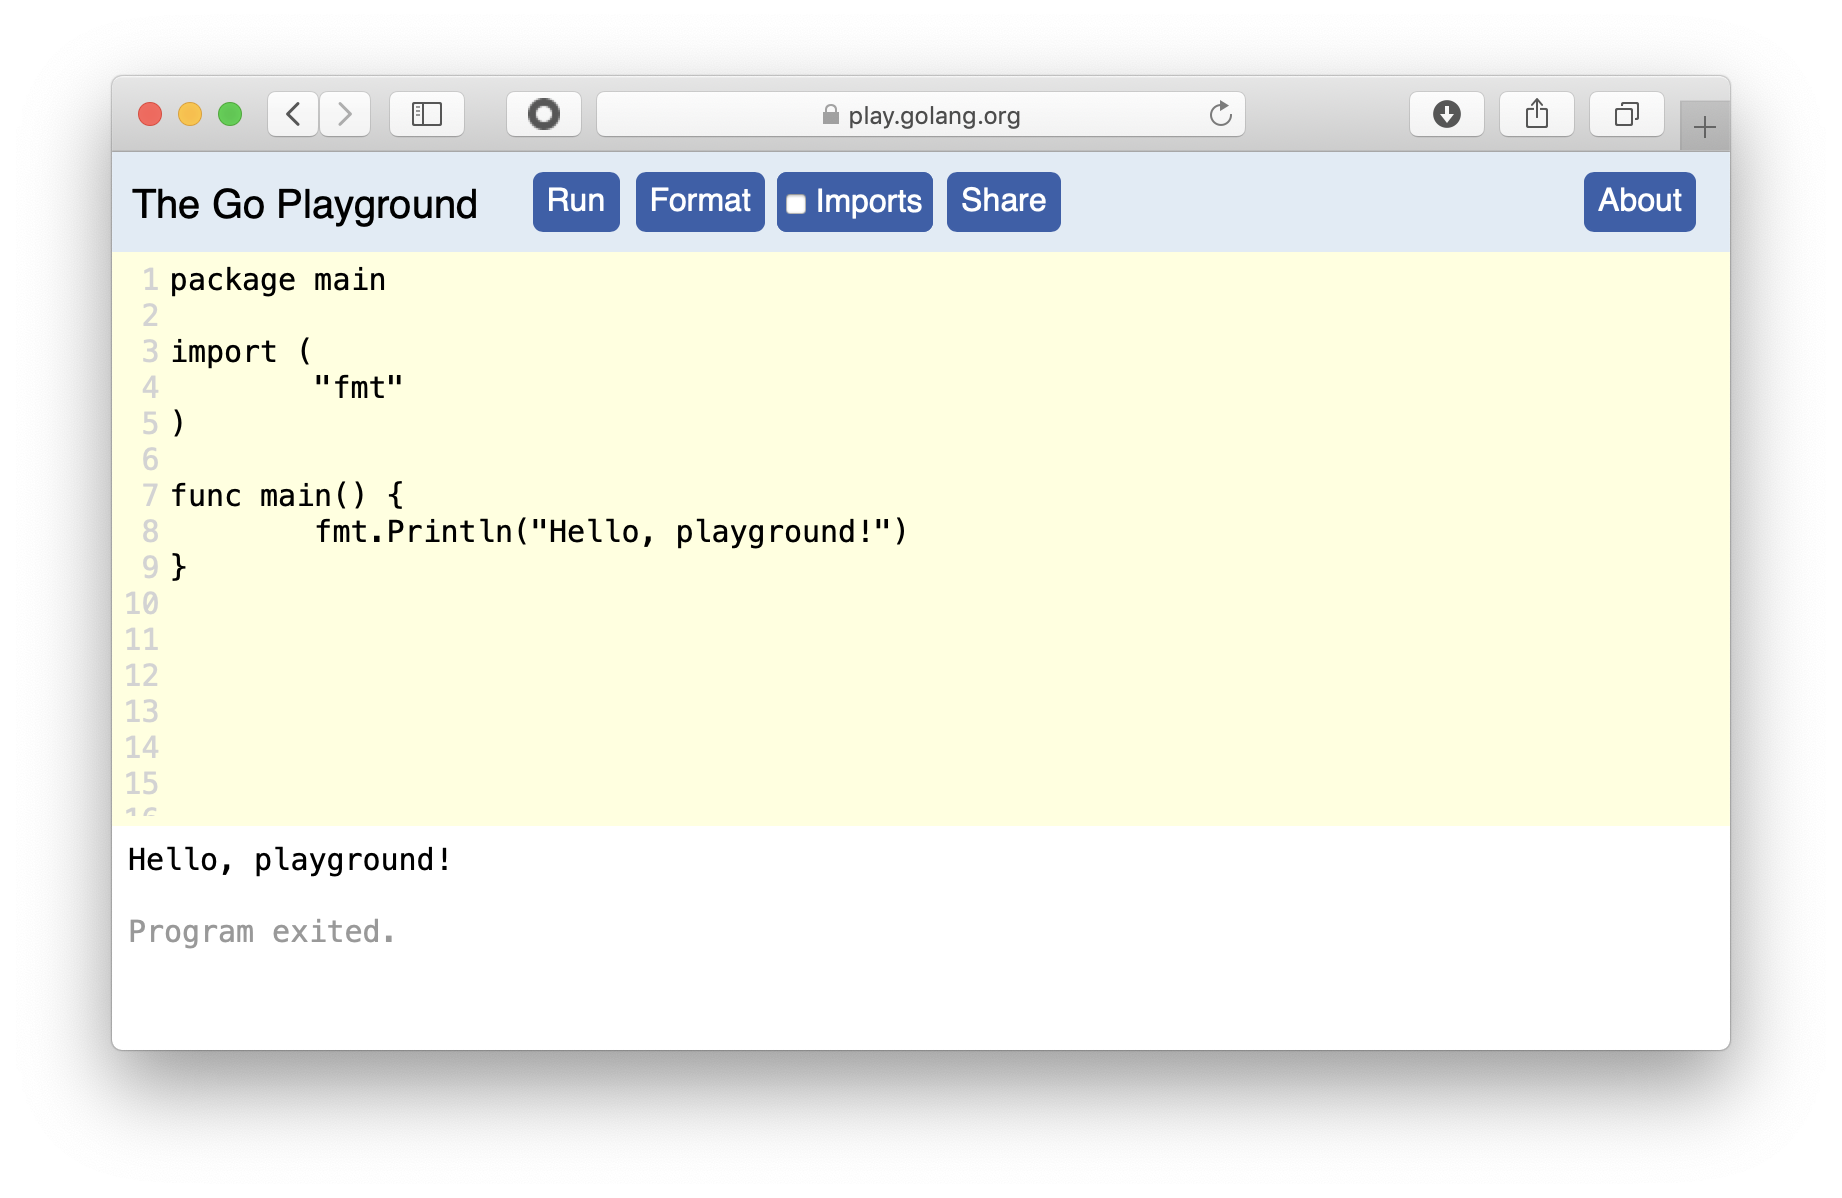
\includegraphics[height=0.9\textheight]{go-playground.png}
\end{center}
\end{frame}

\begin{frame}[fragile]
\frametitle{Hello, world!}
A little more info
\begin{golang}
package main

import "fmt"

func main() {
    fmt.Println("Hello, world!")
}
\end{golang}
    \vspace{0.5\baselineskip}
Notice that semicolons `\verb|;|' aren't normally used in Go \par
    \vspace{0.5\baselineskip}
But everything else here is needed, such as the parentheses \verb|()| for
the function call \par
    \vspace{0.5\baselineskip}
Anything you leave out or misspellll will cause an error
\end{frame}

% \begin{frame}[fragile]
% \frametitle{Compiled vs interpreted}
% A {\em compiler} takes the Go code and converts it to machine
% code that the computer can run \par
%     \vspace{0.5\baselineskip}
% Which means a Go program is fast and efficient \par
%     \vspace{2\baselineskip}
% It also means we need to tell the compiler things about the
% program so it can translate it properly \par
%     \vspace{0.5\baselineskip}
% For example, we need to {\em declare} functions or variables and we
% need to import any package whose functions we want to call \par
%     \vspace{2\baselineskip}
% Interpreted languages can be more flexible but usually aren't as fast
% \end{frame}

\begin{frame}[fragile]
\frametitle{Hello, world!}
Still more info
\begin{golang}
package main

import "fmt"

func main() {
    fmt.Println("Hello, world!")
}
\end{golang}
    \vspace{0.5\baselineskip}
To call a function from a package, we must write the package name
and then a dot `\verb|.|' and then the function name \par
    \vspace{0.5\baselineskip}
The function must have the correct number of arguments in order \par
    \vspace{0.5\baselineskip}
{\em Literal strings} are text sequences in double quotes \verb|""|
\end{frame}

\begin{frame}[fragile]
\frametitle{More strings}
Strings may have {\em escaped} characters
\begin{golang}
package main

import "fmt"

func main() {
    fmt.Println("A string with \"quotes\" inside")
}
\end{golang}
    \vspace{1.5\baselineskip}
The backslash `\verb|\|' is used to {\em escape} a special character \par
    \vspace{0.5\baselineskip}
A \verb|\n| prints a new line, while \verb|\t| prints a tab \par
    \vspace{0.5\baselineskip}
Use two backslashes \verb|\\| to print an actual backslash character
\end{frame}

\begin{frame}[fragile]
\frametitle{Declaring variables}
This code example declares a variable and then assigns
to it later
\begin{golang}
var x int

x = len("a string")
\end{golang}
\vspace{0.5\baselineskip}
But often it's more convenient to use a {\em short declaration} with \\
the \verb|:=| operator
\begin{golang}
x := len("a string")
\end{golang}
    \vspace{0.5\baselineskip}
In both cases \verb|x| is an {\em integer} (it holds whole numbers) \par
    \vspace{0.5\baselineskip}
The first example gave the {\em type} explicitly; in the second, the type
is determined by what \verb|len()| returns
\end{frame}

% \begin{frame}[fragile]
% \frametitle{Variable types}
% Every variable must have a ``static'' type defined in the code
% \begin{itemize}
%     \item numbers might be integers or floating point
%     \item strings are another type
% \end{itemize}
%     \vspace{\baselineskip}
% Number types have an implicit or explicit size
% \begin{itemize}
%     \item \verb|int| is an integer of ``default'' size
%     \item all floats have an explicit size, \verb|float32| or \verb|float64|
% \end{itemize}
%     \vspace{\baselineskip}
% The sizes relate to the number of {\em bits} (binary digits) needed: \par
% \begin{tabular}{rl}
% 8 bits & numbers -128 to 127 (or 0 to 255 if {\em unsigned}\:) \\
% 32 bits & numbers from -2147483648 to 2147483647
% \end{tabular}
% \end{frame}

\begin{frame}[fragile]
\frametitle{Variable names}
Names may contain letters \& digits, and must begin with a letter
\begin{golang}
short
shortName            // capitalize inner words

short_name           // not Go style
SHORT_NAME           // ditto
SHORTNAME            // ditto

name12               // OK
12name               // not allowed
\end{golang}
\end{frame}

\begin{frame}[fragile]
    \frametitle{Integer types}
    Go has a variety of hardware-related integer types
    \begin{itemize}
        \item ``unsized'' (defaults to the machine's natural wordsize): \\
        \verb|int|, \verb|uint| \\
        \vspace{0.5\baselineskip}
        \begin{itemize}
        \item on my Core i7 laptop, these are 64 bits in size
        \item on my Raspberry Pi, these are 32 bits in size
        \end{itemize}
        \vspace{0.5\baselineskip}
        \verb|int| is the default type for integers in Go, even lengths
        \vspace{\baselineskip}
        \item sized, signed: \\
        \verb|int8 int16 int32 int64|
        \vspace{\baselineskip}
        \item sized, unsigned: \\
        \verb|uint8 uint16 uint32 uint64 uintptr|
    \end{itemize}
\end{frame}

\begin{frame}[fragile]
    \frametitle{Other types}
    The \verb|bool| (boolean) type has two values: \verb|false|, \verb|true| \par
        \vspace{0.5\baselineskip}
    These values are {\bf not} convertible to/from integers! \par
        \vspace{2\baselineskip}
    Integer values can't be combined unless they have the same type \par
\begin{golang}
var b bool
var x int16
var y int32

z := x + y           // compile error, type mismatch

z := int32(x) + y    // this is OK

z := int32(b) + y    // this is not allowed
\end{golang}
\end{frame}

\begin{frame}[fragile]
    \frametitle{Declarations are forever}
    Once a variable is declared, its type can't change
\begin{golang}
var x int = 12

x = "a string"       // compile error, type mismatch
x = uint(12)         // ditto
\end{golang}
\vspace{0.5\baselineskip}
This is also true when short declarations are used
\begin{golang}
y := 12              // defaults to type "int"
y = 13               // OK

y = uint(12)         // not OK, type mismatch
y := 13              // not OK, already declared
\end{golang}
\vspace{0.5\baselineskip}
The \verb|:=| operator should not be confused with assignment (\verb|=|)
\end{frame}

\begin{frame}[fragile]
    \frametitle{String-related types}
    Types related to strings:
    \begin{itemize}
        \item \verb|byte|: a synonym for \verb|uint8| \\
        \vspace{0.5\baselineskip}

        \item \verb|rune|: a synonym for \verb|int32| for characters \\
        \vspace{0.5\baselineskip}

        \item \verb|string|: an immutable sequence of ``characters'' \\
        \begin{itemize}
        \item physically a sequence of \verb|byte|
        \item logically a sequence of \verb|rune|
        \end{itemize}
    \end{itemize}
    \vspace{\baselineskip}
    Runes (characters) are enclosed in single quotes: \verb|'a'| \par
    \vspace{\baselineskip}
    ``Raw'' strings use backtick quotes: \verb|`string with "quotes"`| \par
    \vspace{0.4\baselineskip}
    They also don't evaluate escape characters such as \verb|\n|
\end{frame}

\begin{frame}[fragile]
    \frametitle{String-related types}
    Let's see \verb|rune| vs \verb|byte| in a string:
\begin{golang}
package main
import "fmt"

func main() {
    s := "élite"
	fmt.Printf("%8T %[1]v\n", s)
	fmt.Printf("%8T %[1]v\n", []rune(s))
	fmt.Printf("%8T %[1]v\n", []byte(s))
}
\end{golang}
\vspace{0.5\baselineskip}
{\bf é} is one rune (character) but two bytes in UTF-8 encoding:
\begin{verbatim}
  string élite
 []int32 [233 108 105 116 101]
 []uint8 [195 169 108 105 116 101]
\end{verbatim}
\end{frame}

\begin{frame}[fragile]
\frametitle{String-related types, in Chinese}
I can't do this in the slides:
    \vspace{-0.4\baselineskip}
\begin{center}
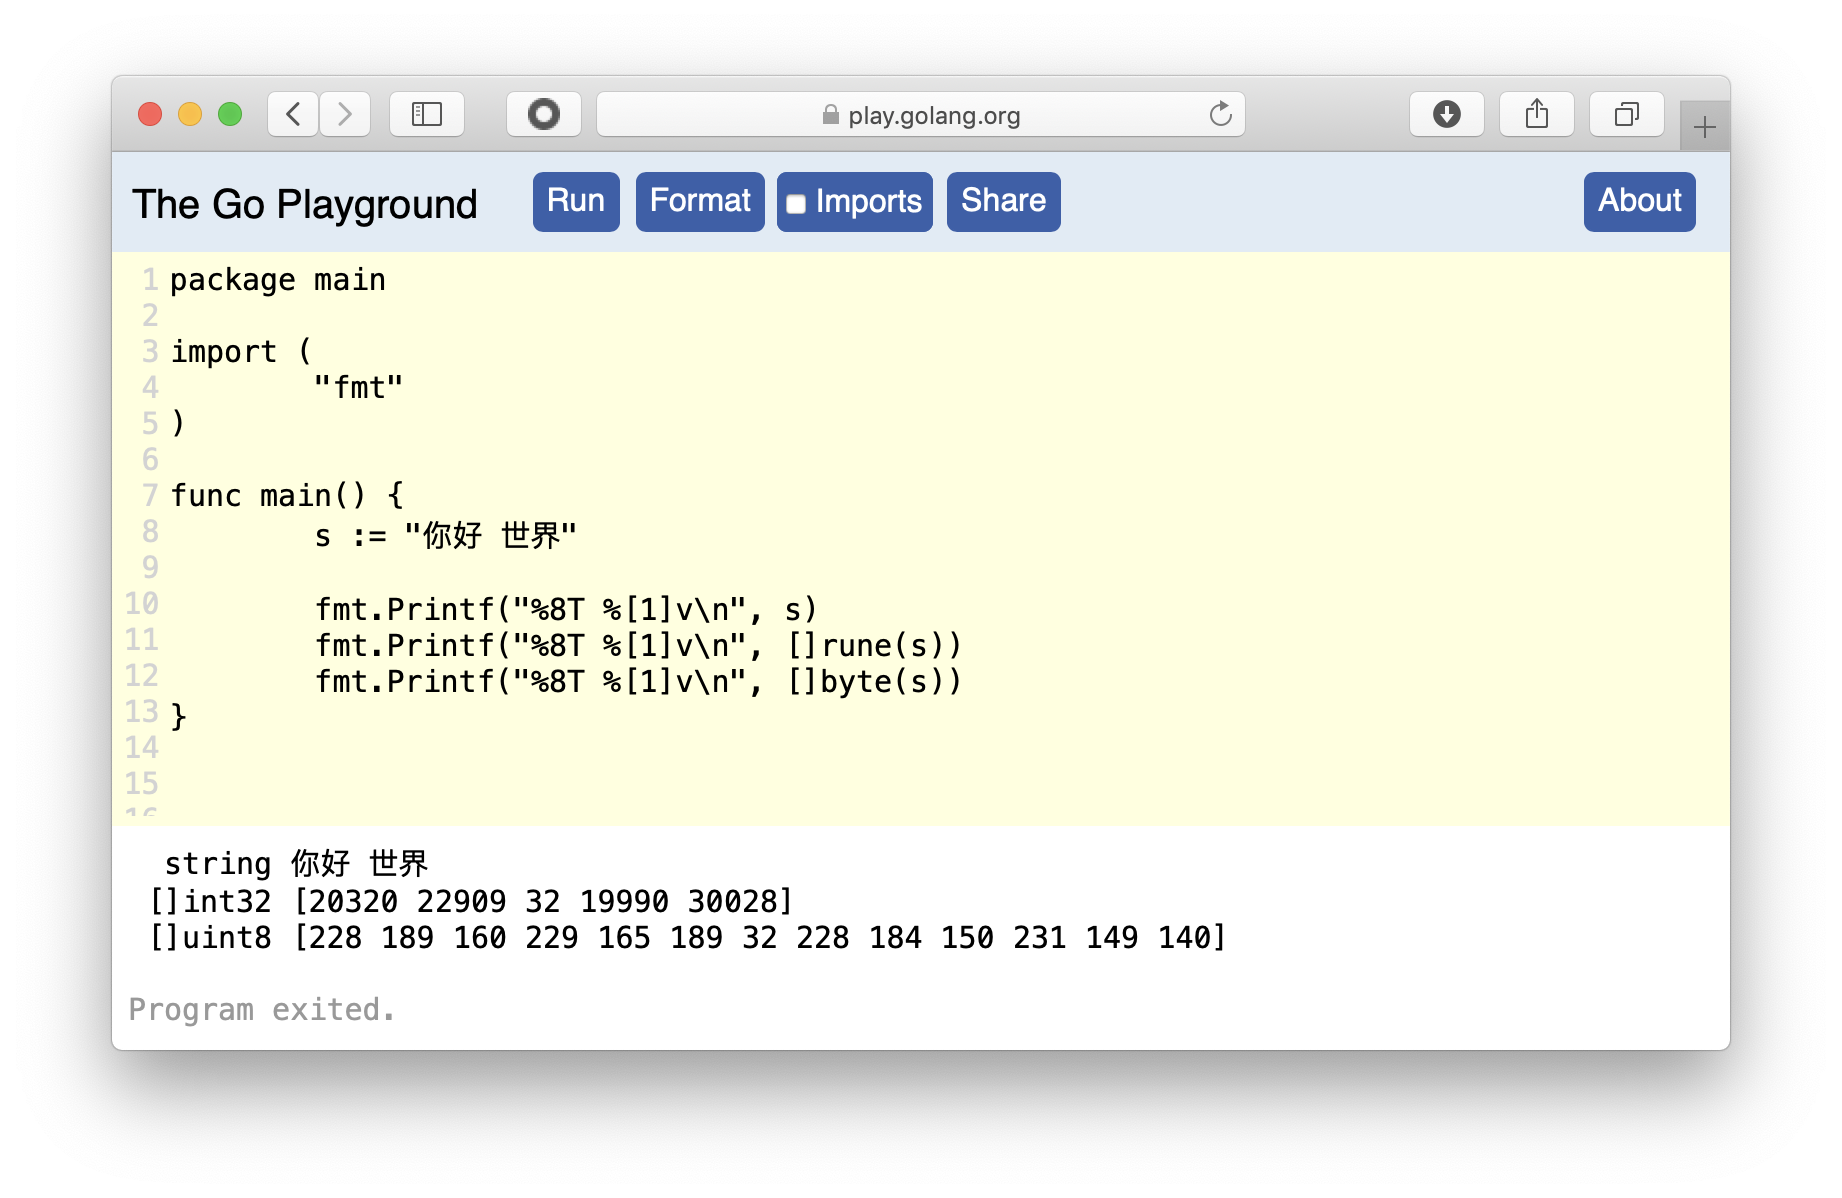
\includegraphics[height=0.9\textheight]{go-playground-chinese.png}
\end{center}
\end{frame}

\begin{frame}[fragile]
    \frametitle{Slices}
    Wait --- what where the \verb|[]| things? \par
    \vspace{2\baselineskip}
    A {\em slice} \verb|[]T| is a {\em sequence} of zero or more \verb|T| \par
    \vspace{\baselineskip}
    A slice of $n$ objects has {\em indexes} $0$ up to \alert{$n-1$}; in math, \alert{$[0,n)$} \par
    \vspace{\baselineskip}
    A slice \verb|x| can be indexed \verb|x[0]| to yield a single item \par
    \vspace{\baselineskip}
    Or it can be indexed \verb|x[m:n]| to yield a slice of \alert{$n-m$} items \\
    (with index values $m$ up to $n-1$) \par
    \vspace{1.2\baselineskip}
    Strings can also use the index brackets to select bytes \par
\end{frame}

\begin{frame}[fragile]
    \frametitle{Slices}
\begin{golang}
package main
import "fmt"

func main() {
	t := []byte("string")   // 0:s 1:t 2:r 3:i 4:n 5:g

	fmt.Println(len(t), t)  // 6 bytes in t
	fmt.Println(t[2])       //   1 item
	fmt.Println(t[:2])      //   2 items
	fmt.Println(t[2:])      // 6-2 items
	fmt.Println(t[3:5])     // 5-3 items
}
\end{golang}
{\small\begin{verbatim}
6 [115 116 114 105 110 103]
114
[115 116]
[114 105 110 103]
[105 110]
\end{verbatim}}
\end{frame}

\begin{frame}[fragile]
    \frametitle{String operations}
    Strings are immutable but can be combined
\begin{golang}
func main() {
    s1 := "a string"
    s2 := "another string"

    fmt.Println(s1 + ", " + s2)

    s3 := s2 + string('?') // can't add a rune

    fmt.Println(s3)
}
\end{golang}
\vspace{\baselineskip}
which produces
\begin{verbatim}
a string, another string
another string?
\end{verbatim}
\end{frame}

\begin{frame}[fragile]
    \frametitle{String functions}
    Package \verb|strings| has many functions on strings
\begin{golang}
s := "a string"

x := len(s)                 // built-in, = 8

strings.Contains(s, "g")    // returns true
strings.Contains(s, "x")    // returns false

strings.HasPrefix(s, "a")   // returns true
strings.ToUpper(s)          // returns "A STRING"
\end{golang}
\vspace{1.5\baselineskip}
Indexes in strings are numbered from \verb|0| up to \verb|len(s) - 1|
\begin{golang}
strings.Index(s, "string")  // returns 2
\end{golang}
\end{frame}

%% ================================================================================

\section{Program Logic}
\begin{frame}[fragile]
    \frametitle{The logic of a program}
    Programs don't just have variables, they need logic \par
    \vspace{0.5\baselineskip}
    There are three main kinds of logic structures:
    
    \begin{description}[labelwidth=\widthof{\bfseries \:\:separating out pieces of logic:},align=right]
    \item [{\color{black} making choices:}] if-then-else
    \item [{\color{black} repeating things:}] loops
    \item [{\color{black} separating out pieces of logic:}] functions
    \end{description}
    \vspace{\baselineskip}
    In the absence of other structure, execution proceeds from top to bottom:
\begin{golang}
func main() {
    doThisFirst()
    thenDoThis()
}
\end{golang}
\end{frame}

\begin{frame}[fragile]
    \frametitle{Alternation}
    ``If it's sunny, we'll go to the ballgame, otherwise a movie'' \par
    \vspace{0.5\baselineskip}
    That same type of logic is applied using the ``if-then-else'' structure
\begin{golang}
func main() {
    weather := os.Args[1]     // command-line arguments

    if weather == "sunny" {
        doGame()
    } else {
        doMovie()
    }
}
\end{golang}
    \vspace{0.5\baselineskip}
The if-condition is a {\em boolean} expression which must evaluate
to either \verb|false| or \verb|true|
\end{frame}

\begin{frame}[fragile]
    \frametitle{Boolean and conditional operators}
    Conditions include the notion of ``equal to'' for most types: \par
    \vspace{-0.2\baselineskip}
\begin{description}[labelwidth=1in,align=right]
\item [{\color{black}{\tt ==}}] equal to
\item [{\color{black}{\tt !=}}] not equal to
\end{description}
    \vspace{0.5\baselineskip}
Only strings and numbers normally have order:
    \vspace{-0.2\baselineskip}
\begin{description}[labelwidth=1in,align=right]
\item [{\color{black}{\tt \:\:<}}] less than
\item [{\color{black}{\tt <=}}] less than or equal to
\item [{\color{black}{\tt \:\:>}}] greater than
\item [{\color{black}{\tt >=}}] greater than or equal to
\end{description}
    \vspace{1.5\baselineskip}
\verb|=| means assigment, not equality, while \verb|:=| is a short declaration
\end{frame}

\begin{frame}[fragile]
    \frametitle{Boolean and conditional operators}
    Conditions can be combined with boolean operators: \par
    \vspace{-0.2\baselineskip}
\begin{description}[labelwidth=1in,align=right]
\item [{\color{black}{\tt \&\&}}] and
\item [{\color{black}{\tt ||}}] or
\item [{\color{black}{\tt \:\:!}}] not (as a prefix)
\end{description}
\begin{golang}
    x < y || x < z  // x must be less than one of y, z
    n > 0 && !b     // n must be positive and b not true
\end{golang}
    \vspace{\baselineskip}
\verb|&&| and \verb$||$ are {\em shortcut} operators; they evaluate the
right side only \\if necessary \par
\vspace{0.5\baselineskip}
For example, if \verb|x| is 0, we know this expression is false just from its left side:
\vspace{-0.5\baselineskip}
\begin{golang}
    x != 0 && y/x >= 1
\end{golang}
\end{frame}

\begin{frame}[fragile]
    \frametitle{Repetition}
    ``Print the line ten times'' \par
    \vspace{0.5\baselineskip}
    The ``for'' loop is called that because most often it looks like
\begin{golang}
func main() {
	s := "I will not talk in class"

	for i := 0; i < 10; i++ {
		fmt.Println(s)
	}
}
\end{golang}
\vspace{0.5\baselineskip}
The parts separated by `\verb|;|' are
\begin{itemize}
    \item a short declaration of a {\em loop index}
    \item a repeating condition (do the {\em loop body} while true)
    \item an expression changing the loop index (after the body)
\end{itemize}
\end{frame}

\begin{frame}[fragile]
    \frametitle{Repetition}
    ``Roll the dough until it is smooth'' \par
    \vspace{0.5\baselineskip}
    The loop control can be just a boolean expression:
\begin{golang}
func main() {
    d := makeDough()

    for !d.smooth() {
        d.roll()       // must set smooth() true sometime
    }
    
    bake(d)
}
\end{golang}
    \vspace{0.5\baselineskip}
Go only has one loop structure (there's no ``while'' or ``until''), but it
does have some additional options
\end{frame}

\begin{frame}[fragile]
    \frametitle{Repetition}
    ``For all values in the sequence, do this'' \par
    \vspace{0.5\baselineskip}
    The \verb|range| operator ranges over a sequence, returning an index and a value:
\begin{golang}
func main() {
    s := "abc"

    for i, r := range s {
        fmt.Println(i, r, string(r))
    }
}
\end{golang}
\vspace{0.5\baselineskip}
\begin{verbatim}
0 97 a
1 98 b
2 99 c
\end{verbatim}
\end{frame}

\begin{frame}[fragile]
    \frametitle{Repetition}
    ``Do this forever'' \par
    \vspace{0.5\baselineskip}
    This loop will run until \verb|break| makes it stop
\begin{golang}
func main() {
    scanner := bufio.NewScanner(os.Stdin)

    for {
        if !scanner.Scan() {
            break
        }

        fmt.Println(scanner.Text())
    }
}
\end{golang}
    \vspace{0.5\baselineskip}
Here \verb|Scan()| will return \verb|false| only if there's no more input
\end{frame}

\begin{frame}[fragile]
    \frametitle{A complete repeating program}
\begin{golang}
package main
import ("fmt"; "bufio"; "os")   // legal, bad style

func main() {
    scanner := bufio.NewScanner(os.Stdin)

    for {
        fmt.Print("Enter your text: ")
        ok, text := scanner.Scan(), scanner.Text()

        if !ok || text == "q" {
            fmt.Println()
            break
        }

        fmt.Println("Your text was: ", text)
    }
}
\end{golang}
\end{frame}

\begin{frame}[fragile]
    \frametitle{Functions}
    We've already created one function: \verb|main| \par
    \vspace{2\baselineskip}
    Often we have some code we don't want to retype over \& over \par
    \vspace{0.5\baselineskip}
    If we put it into a function, it's reusable \par
    \vspace{2\baselineskip}
    Breaking up big programs into functions make them easier to read \par
    \vspace{0.5\baselineskip}
    And think about
\end{frame}

\begin{frame}[fragile]
    \frametitle{Functions}
    Most functions take {\em parameters} (or ``arguments'') as input \par
    \vspace{0.5\baselineskip}
    And possibly give back a {\em return value}
\begin{golang}
func twice(x int) int {    // twice(10) will be 20
    return 2 * x
}
\end{golang}
    \vspace{0.8\baselineskip}
OK, that was lame; how about
\begin{golang}
func quadratic(a, b, c float64) (float, float) {
    d := math.Sqrt(b*b - 4*a*c)
    return (-b + d)/(2*a), (-b - d)/(2*a)
}
\end{golang}
    \vspace{0.6\baselineskip}
Yes, a function can return more than one value
\end{frame}

\begin{frame}[fragile]
    \frametitle{Functions}
    We've been calling a bunch of functions so far \par
    \vspace{0.5\baselineskip}
\begin{golang}
s := "a string"

strings.ToUpper(s)         // returns "A STRING"
strings.Contains(s, "a")   // returns true

x := 16.0

math.Sqrt(x)               // returns 4.0
\end{golang}
    \vspace{0.5\baselineskip}
Note that we must write \verb|16.0| or \verb|x| will be an \verb|int| \par
    \vspace{2\baselineskip}
Why does that matter?
\end{frame}

\begin{frame}[fragile]
    \frametitle{Function parameters}
    Every function parameter has a name and a type \par
    \vspace{0.5\baselineskip}
    To call a function, the {\em actual} parameters must match the
    all the {\em formal} parameters in the correct order
\begin{golang}
func friz(a int, b string)

friz(2, "a")               // OK

frize(2.0, "x")            // wrong type for "a"
friz(2, 1)                 // wrong type for "b"
friz(2)                    // not enough parameters
\end{golang}
    \vspace{\baselineskip}
\verb|math.Sqrt()| takes a floating point number, not an integer
\begin{golang}
func Sqrt(x float64) float64
\end{golang}
\end{frame}

\begin{frame}[fragile]
    \frametitle{Methods}
    Some functions are {\em methods} because we call them on an object \par
    \vspace{0.5\baselineskip}
    They're just a special type of function call
\begin{golang}
package main

import ("fmt"; "bufio"; "os")

func main() {
    scanner := bufio.NewScanner(os.Stdin)    // function

    scanner.Scan()                           // method
    fmt.Println("That's ", scanner.Text())   // one of each
}
\end{golang}
    \vspace{\baselineskip}
We qualify the function with the object name, not a package name
\end{frame}

%% ================================================================================
\section{Tools and Techniques}
\begin{frame}[fragile]
    \frametitle{Installation}
    Start from the Go language page: \href{https://golang.org}{https://golang.org} \par
    \vspace{0.5\baselineskip}
    {\bf Mac}: run \verb|brew install go| (or use the installer package) \par
    {\scriptsize Homebrew installation: \href{https://brew.sh}{https://brew.sh}} \par
    \vspace{0.75\baselineskip}
    {\bf Windows}: open the installer (MSI) file and follow the prompts to install the Go tools \par
    {\scriptsize(otherwise you can download a ZIP file, but you have to set some environment stuff)} \par
    \vspace{0.75\baselineskip}
    {\bf Linux}: download the archive and extract it into \verb|/usr/local|, \\
    creating a Go tree in \verb|/usr/local/go| \\
    \vspace{0.5\baselineskip}
    {\scriptsize\verb|sudo tar -C /usr/local -xzf go1.11.5.linux-amd64.tar.gz|} \\
    \vspace{0.5\baselineskip}
    and don't forget to add \verb|/usr/local/go/bin| to \verb|$PATH| (Linux)\\
\end{frame}

\begin{frame}[fragile]
    \frametitle{Go command-line tools}
    The \verb|go| program can run code or make a binary \par
    \vspace{0.5\baselineskip}
\verb|go run| compiles to a temporary directory, then deletes the result
    \vspace{0.25\baselineskip}
{\small\begin{verbatim}
$ go run hello.go      ## temporary compile
Hello, world!

$ gofmt -w hello.go    ## standard format

$ go build hello.go    ## produces a binary "hello"

$ ./hello
Hello, world!
\end{verbatim}}
    \vspace{0.5\baselineskip}
    \verb|gofmt| reformats code, use the \verb|-w| option to overwrite the file
\end{frame}

\begin{frame}[fragile]
\frametitle{Printing command-line arguments}
\begin{golang}
package main

import ("fmt"; "os")

func main() {
    var s, sep string

    for i := 1; i < len(os.Args); i++ {
        s += sep + os.Args[i]
        sep = " "
    }

    fmt.Println(s)
}
\end{golang}
    \vspace{0.25\baselineskip}
We'll skip \verb|os.Args[0]| because that's the program name:
{\tiny \verb|/var/folders/6y/q8z5w4xn1dzb0_qz680mcs6h0000gn/T/go-build451715571/b001/exe/hello|}
\end{frame}

\begin{frame}[fragile]
    \frametitle{Running a program with a bug}
    Here's a short program:
\begin{golang}
func main() {
    fmt.Println(os.Args[1])
}
\end{golang}
    \vspace{0.5\baselineskip}
    Running it on the command line: \par
    \vspace{0.5\baselineskip}
    {\small\tt \$ go run badargs.go \:\:\: \alert{\#\# no argument given} \\
    panic: runtime error: index out of range \\

    goroutine 1 [running]: \\
    main.main() \\
        /Users/mholiday/go/src/badargs/badargs.go:55 +0x202 \\
    exit status 2 }\\
    \vspace{\baselineskip}
    What went wrong? We read past the end of \verb|os.Args|! \par
\end{frame}

\begin{frame}[fragile]
    \frametitle{Reading a file}
    Here's another program that checks a file's size
\begin{golang}
package main

import ("fmt"; "io/ioutil"; "os")

func main() {
    fname := os.Args[1]
    if f, err := os.Open(fname); err != nil {
        fmt.Fprintln(os.Stderr, "bad file:", err)
    } else if d, err := ioutil.ReadAll(f); err != nil {
        fmt.Fprintln(os.Stderr, "can't read:", err)
    } else {
        fmt.Printf("The file has %d bytes\n", len(d))
    }
}
\end{golang}
If run on itself (the source file), it prints ``The file has 333 bytes''
\end{frame}

\begin{frame}[fragile]
    \frametitle{Reading a file}
    Wait, what's going on here?
\begin{golang}
if f, err := os.Open(fname); err != nil {
    fmt.Fprintln(os.Stderr, "bad file:", err)
} . . .
\end{golang}
    \vspace{0.5\baselineskip}
An if-statement can have a short declaration as its first part \par
    \vspace{\baselineskip}
We often call functions whose 2nd return value is a possible error \par
\begin{golang}
    func Open(name string) (*File, error)
\end{golang}
where the \verb|error| can be compared to \verb|nil|, meaning no error \par
    \vspace{\baselineskip}
\alert{\bf Always check the error} --- the file might not really be open! \par
\end{frame}

%% ================================================================================

\section{Homework}
\begin{frame}[fragile]
    \frametitle{Homework \# 1}
    Write a program to take a file name from the command line \\
    and count the lines in the file (a line ends with \verb|"\n"|). \par
    \vspace{2\baselineskip}
    You can test your first program with \verb|wc|: \par
    \vspace{-0.2\baselineskip}
    {\scriptsize
\begin{verbatim}
  $ wc testing.txt
         9      35     180 testing.txt
\end{verbatim}} \par
    which prints out the number of lines, words, and characters \par
    \vspace{2\baselineskip}
    You may want to use \verb|scanner.Scan()| and \verb|scanner.Text()|
\end{frame}

\end{document}
